\chapter{Architecture in Distributed Applications}
\label{ch:architecture}

\textit{Identifying the optimal architecture for a system is extremely important, as it has a major influence in all factors of a software project throughout: development, deployment, expansion and maintenance of the system. This chapter will follow up on the previous case description and explain the evolution of software architecture, elaborating on three fundamentally different ways of structuring software projects}

Considering the architecture of any system is extremely important to ensure that the application can be effectively developed, deployed and expanded in the future. Architecture for distributed applications has moved through three main phases: monolith, service oriented architecture (SOA), and currently Microservice is gaining a lot of attention. Each iteration of architecture has learned valuable lessons from the latter, with an increasing focus on breaking a system into lesser parts, simplifying working with the system at hand. According to Martin Fowler the term architecture has many meanings, but two common elements \cite[p.~1]{fowler2002patterns}:

Breaking the system into smaller parts makes it easier to comprehend possible solutions and structure code.

Many external factors influence how software has been developed through time, available languages, frameworks and tools has drastically changed how software is developed today. 

Competition has also had it's influence by setting new requirements to the speed of development, having short and agile release cycles has never been more important.

At the same time users have gained a more intricate knowledge of software and the possibilities having high expectations for functionality and consistency of the software that is developed.


\note {
Monolith gives good inter-module re-factoring capabilities. If you want to change a boundary, you can easily change it. When using microservices it is hard to change interfaces when they are in place. Therefore it is not advised to start out with a microservice architecture if the module boundaries well are not well known.

Monolith makes it to easy to run around modularity. Not keeping module boundaries solid. 

In many ways microservices are a discipline that forces you to keep your modularity.

Microservices allow you to use multiple platforms, gives flexibility. 

Monolith are simple to use, because we are used to doing it that way. Microservices are so cool, we want to do it. If you look at an application and say it would work nice as a single rails service, then do not do microservices. They introduce distributed computing, asynchronous communication, they are hard to do \cite{fowler2014microservicesoamonolith}.
}

\note {

\cite{fowler2017what} "The value of a Patterns is saying here is a specific technique, some ideas about when it is applicable or not and enough knowledge about a pattern to know: these are the things i should watch out for these are some of the things that I would expect to see as consequences of that."
"Saying something as vague as event-driven is too imprecise, similar problems exist with SOA, it mean so many different things"

"Microservices carve down what it is about"

}

\note{
“ This chapter is about architectural styles, application architectures, and architecture patterns. A style describes how to implement a specific architecture, while an architecture pattern explains how to address a specific concern within an architecture but is broader than a design pattern. I suggest you not get too hung up on the differences, but just understand that DDD can reside at the heart of a lot of surrounding architectural influences.”
Excerpt From: Vernon, Vaughn. “Implementing Domain-Driven Design.”

We need to emphasize that there are many ways of doing architecture and many reason for doing particular architectures. Functional and non-functional requirements
}


\section{Defining Architecture in Distributed Systems}


\defi{Architecture (Oxford)}{The conceptual structure and logical organization of a computer or computer-based system}{\url{https://en.oxforddictionaries.com/definition/architecture}}

It is important to establish the abstraction level when talking about software development, when developing distributed applications every level should be incorporated in the discussion, as each level has different implications for the final application.



When designing distributed applications two main levels exist: Application and Infrastructure. The application level is the lower level where application definition and development take place, here many decisions have to be made taking developer competences, organisation and process among other factors into account. Which languages and frameworks are available, which database fit the data best, which subversion tool can be utilized, how are dependencies defined and managed, is it necessary to deploy any Continuous Integration (CI) or Continous Delivery (CD) tools and how do we manage the applications external API?. 

Decisions on this level will influence the application throughout it's entire lifetime, from development through to deployment and possibly in the end retirement. Some decisions are easier to change than others, Nygaard state the following about decoupling middleware, showing how crucial basic architectural decisions can be \cite[p.~116]{nygard2007release}:

\tquote{Decoupling Middleware is an architecture decision. It Ripples into every part of the system. This is one of those nearly irreversible decisions that should be made early rather than late}{Nygaard}{2007}

Some application level architecture decisions ripple into every part of the application, while others causes minor changes in parts of the system. Being aware of the implications of a certain architecture is crucial.



"A microservice architecture is the natural consequence of applying the single responsibility principle at the architectural level. This results in a number of benefits over a traditional monolithic architecture such as independent deployability, language, platform and technology independence for different components, distinct axes of scalability and increased architectural flexibility."\cite[p.~3]{fowler2014testing}


\section{Domain Driven Design}
\label{sec:DDD}
The DDD term was coined by Eric Evans in his book of the same name from 2004\cite[preface]{evans2004domain}. Evans works with the notion that any complex domain should be partitioned into smaller subdomains, making it possible to comprehend the different subdomains and how a good solution can be created in that part of the domain. Models express a deep understanding of a particular subdomain, defining a model makes it possible to talk about the domain internal in a development team and externally with other development teams or customers. The model is a product of careful analysis of the domain, and should be reflected in the implementation, so that the analysis of the domain is visible in the code. This makes it possible to understand the implementation, and helps when maintaining and updating the application\cite[p.~2]{evans2004domain}.

Evans deems it very important that a model is kept simple, emphasizing the need for having several subdomains with their own model. Having a single model for a large system is not feasible or cost-effective\cite[p.~331]{evans2004domain}. By introducing what he calls \textit{Bounded contexts}, a models applicability is limited. A model is created in relation to a certain context, and this context will vary between each subdomain, concepts will likely occur in several subdomains, but might have very different meanings. Sharing a model across bounded contexts might hide the fact that there is a discrepancy in how the model is utilized, which can cause buggy and unreliable software, that is hard to understand. By limiting usage of a model, by explicitly defining bounded contexts, teams have a clear understanding of what is consistent across context and how it relates to their context\cite[p.~331]{evans2004domain}. Figure \ref{fig:architecture_bounded_context} show a domain with three bounded contexts and five subdomains. The different subdomains have dependencies across bounded context boundaries, indicating integration points.

\begin{figure}[!htb]
  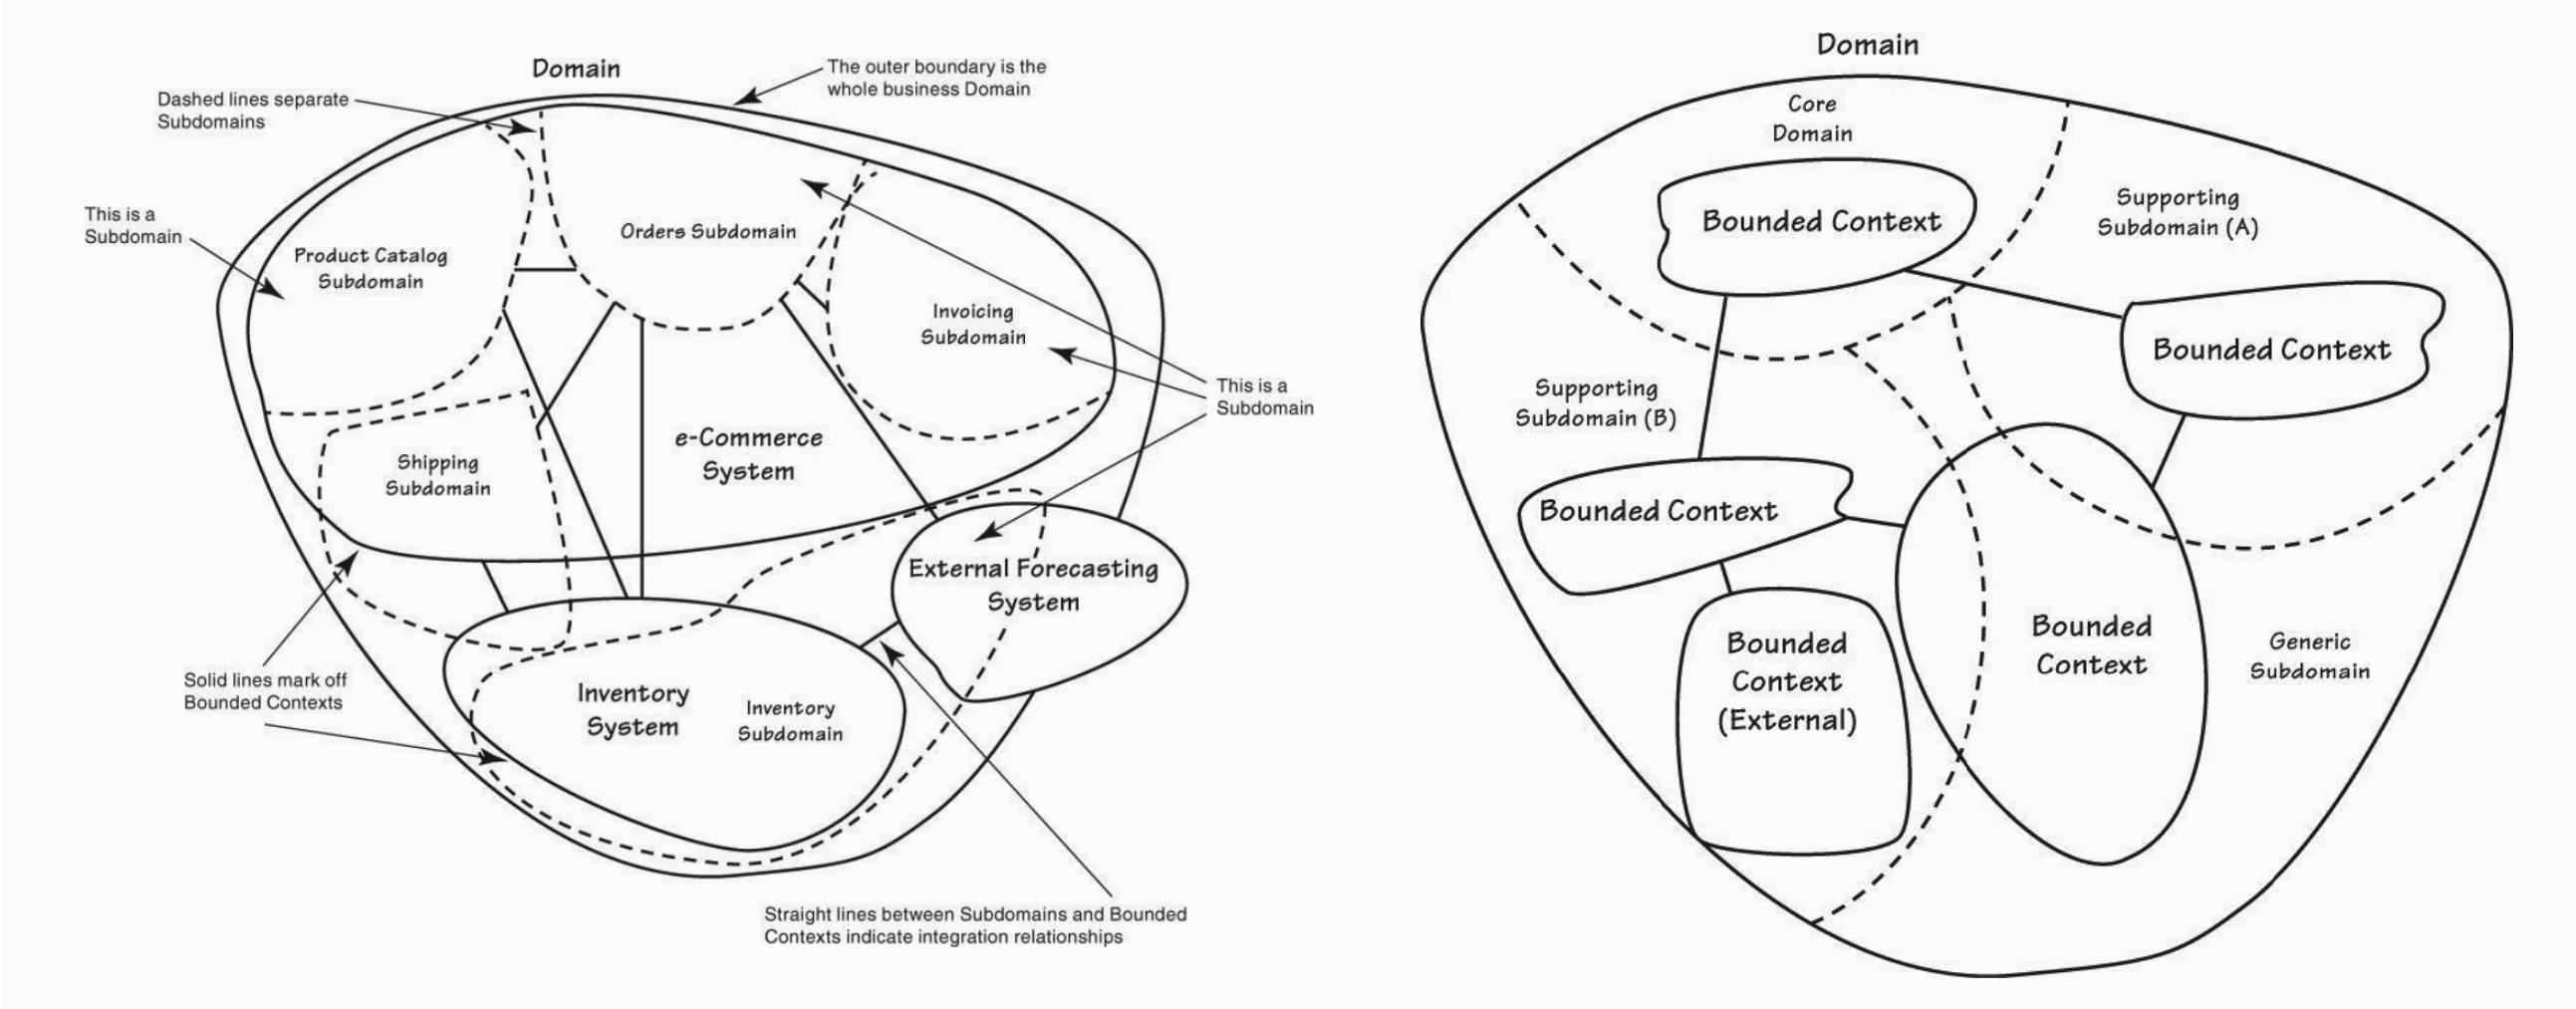
\includegraphics[scale=0.28]{architecture_bounded_context}  
  \caption{An example of bounded context}
  \label{fig:architecture_bounded_context}
\end{figure}


According to Lewis and Fowler\cite{fowler2014microservices} usability of DDD when designing distributed applications are described is:

\tquote{DDD divides a complex domain up into multiple bounded contexts and maps out the relationships between them. This process is useful for both monolithic and microservice architectures, but there is a natural correlation between service and context boundaries that helps clarify, and as we describe in the section on business capabilities, reinforce the separations}{Lewis and Fowler}{2014}

According  emphasize how DDD is usable, generally when designing applications, also mentioning how separation between bounded contexts is more explicit when using microservices, highlighting one of the key features of the architecture. Reducing the risk of sharing model across bounded contexts.

\section{Monolithic}
The word monolith describes a application that exists as an single unit. By having the entire application as a single entity, the source code can be developed and managed together, giving multiple short term advantages\cite[p.~68]{long2017cloud}. Functionality can easily be added on top of a existing code base, giving the many advantages of low level programming language constructs. Communication can be done internally, between processes, not relying on non-deterministic network communication channels. 
According to Lewis and Fowler\cite{fowler2014microservices} enterprise web applications are often created as a monolith, consisting of three main parts: a client-side user interfaces, a shared common database management systems and a monolith server-side applications. The server-side application is a large and complex application, packed into a single executable. The application binds interface and database together, executing domain logic based on user input, retrieving and updating data as needed. 
As the application grows in size, immediate advantages fade. The code base reaches a size where small changes in one part of the application might incur unforeseen changes in other parts. Centralizing the application decreases risk of failure, but at the same time forces development teams to coordinate changes, making sure breaking changes are not introduced\cite[p.~68]{long2017cloud}. 
According to Eric Evans having a single and unified model for a large system is not feasible nor cost-effective, and have several potential pitfalls if legacy code is updated by several teams simultaneously. Coordination might halt the project completely. The unified model may not be sufficient for some parts of the application, forcing functionality in elsewhere. Having a unified model leads to a very complex model that tries to encapsulate all aspects of the particular domain, making it difficult to use and therefore defeating the purpose\cite[p.~331]{evans2004domain}.

\subsection{Netflix -- the Transition away from the Monolith}
According to Meshenberg\cite{meshenberg2016microservices} Netflix previously had a monolithic implementation of their website. Each team would contribute a JAR file, that would be gathered into a single WAR file, that was deployed on a internal infrastructure. According to Meshenberg, this kind of architecture is very unreliable, mentioning that any issue introduced in either of the JAR files would be propagated onto all copies of the single service site executable. More importantly, the old architecture had a single relational database management system (RDBMS), creating a single point of failure\cite{meshenberg2016microservices}. Netflix experienced a outage, where their central RDBMS failed and caused wide system failure, resulting in four days with downtime. According to Meshenberg this event started the Netflix transition from a monolith to a microservice architecture.

\note {
The client-side user interface consists of HTML pages, with some underlying javascript files. The database is a shared among all applications in the enterprise, implemented as a relational database, containing tables for the entire business domain. The server-side application is a monolith, binding interface and database together, executing domain logic based on user input and retrieving and updating data as needed. The server-side application is a single executable.

"To start explaining the microservice style it's useful to compare it to the monolithic style: a monolithic application built as a single unit. Enterprise Applications are often built in three main parts: a client-side user interface (consisting of HTML pages and javascript running in a browser on the user's machine) a database (consisting of many tables inserted into a common, and usually relational, database management system), and a server-side application. The server-side application will handle HTTP requests, execute domain logic, retrieve and update data from the database, and select and populate HTML views to be sent to the browser. This server-side application is a monolith - a single logical executable[2]. Any changes to the system involve building and deploying a new version of the server-side application." \cite{fowler2014microservices}
}


\section{Service-Oriented Architecture}

SOA defines a enterprise services bus (ESB) at it's core, which is a used to send messages between components connected to it. Messages are send to the bus, with attached metadata containing information about the tasks needing to be solved for a given client application. SOA often incorporates a high amount of middleware, sitting between the components connected to the event bus, the middleware registers services connected to the service bus, creating a registry of available services. The middleware can contain business logic, taking several forms, from very industry-specific to more general purpose applications. SOA often utilizes Simple Object Access Protocol (SOAP) for message-passing, passing Extensible Markup Language (XML) documents between services \cite[p.~272]{sosinsky2010cloud}.

Martin Fowler author and Chief Scientist at ThoughtWorks, spoke about microservices at GOTO Berlin 2014 stating the following about the ESB \cite[t.8.15]{fowler2014microservicesoamonolith}:
\tquote{When a lot of people talk about service oriented architecture they talk about the idea of let's get some powerfull piece of middleware that will automatically do all sorts of stuff it will route message it will apply business rules it does all sorts of things, this of course is the enterprise service bus or as it is more correctly know, the egregious spaghetti box}{Fowler}{20015}


Means many things to different people, it is hard to understand what it is.

Comittess that lay down standards for how services connect to each other. SOA is a too broad term, it means so many things that it is effectively useless. Microservices is a subset of the SOA term, it therefore makes sense to say that microservices not necesarrily brings anything new to the table. At the same time a new term makes it possible to concentrate on specific and very usable parts of SOA.

Cooperation that brings downs 

\cite{microsoft2017chapter}

There are many different view on what SOA is and how it is used to develop software. According to 

Focus is not on the specific implementation, but on how the architecture can support our organizations needs and goals. There might be some common infrastructure capabilities of every SOA architecture, but the architecture should match the organisation. 

“Web services enabled a new form of a widely used communication mechanism—a challenger to using the SQL with shared databases. (Much of this work was done under the banner of “Service-Oriented Architecture”—a term most notable for its lack of a consistent meaning.)”

Excerpt From: pramod j. sadalage. “NoSQL Distilled: A Brief Guide to the Emerging World of Polyglot Persistence.” iBooks. 


\section{Microservices}
Microservice architecture gives an application composed of many small intercommunicating services. Each individual service has a well defined and limited functionality and a well defined interface for external communication. Services communicate with each other through their interfaces and together they achieve a overarching business goal\cite[p.~2]{newman2015microservices}. A comparison between a monolithic and microservice architecture is shown on Figure \ref{fig:architecture_microservice_definition}, showing they key difference between the two architecture types. Microservices are independently deployable, whereas the monolith scales 1:1, giving less flexibility. 

Having small and independently deployable services makes it possible to update services as teams identify problems or add new features. This supports agile software development, giving the flexibility and agility that the monolithic implementation lacks. By having small services, creating a modular, easy readable and understandable architecture is easier. Each service can be developed, tested and deployed independently, by the team creating it, minimizing the need for coordination between teams\cite{kniberg2014spotify}.

At the same time microservices introduce more complexity. By having individual services, each service has it's own life cycle and can potentially fail. Microservices makes it necessary to have increased automation when deploying, monitoring and maintaining system health\cite{meshenberg2016microservices}.

\begin{figure}[!htb]
  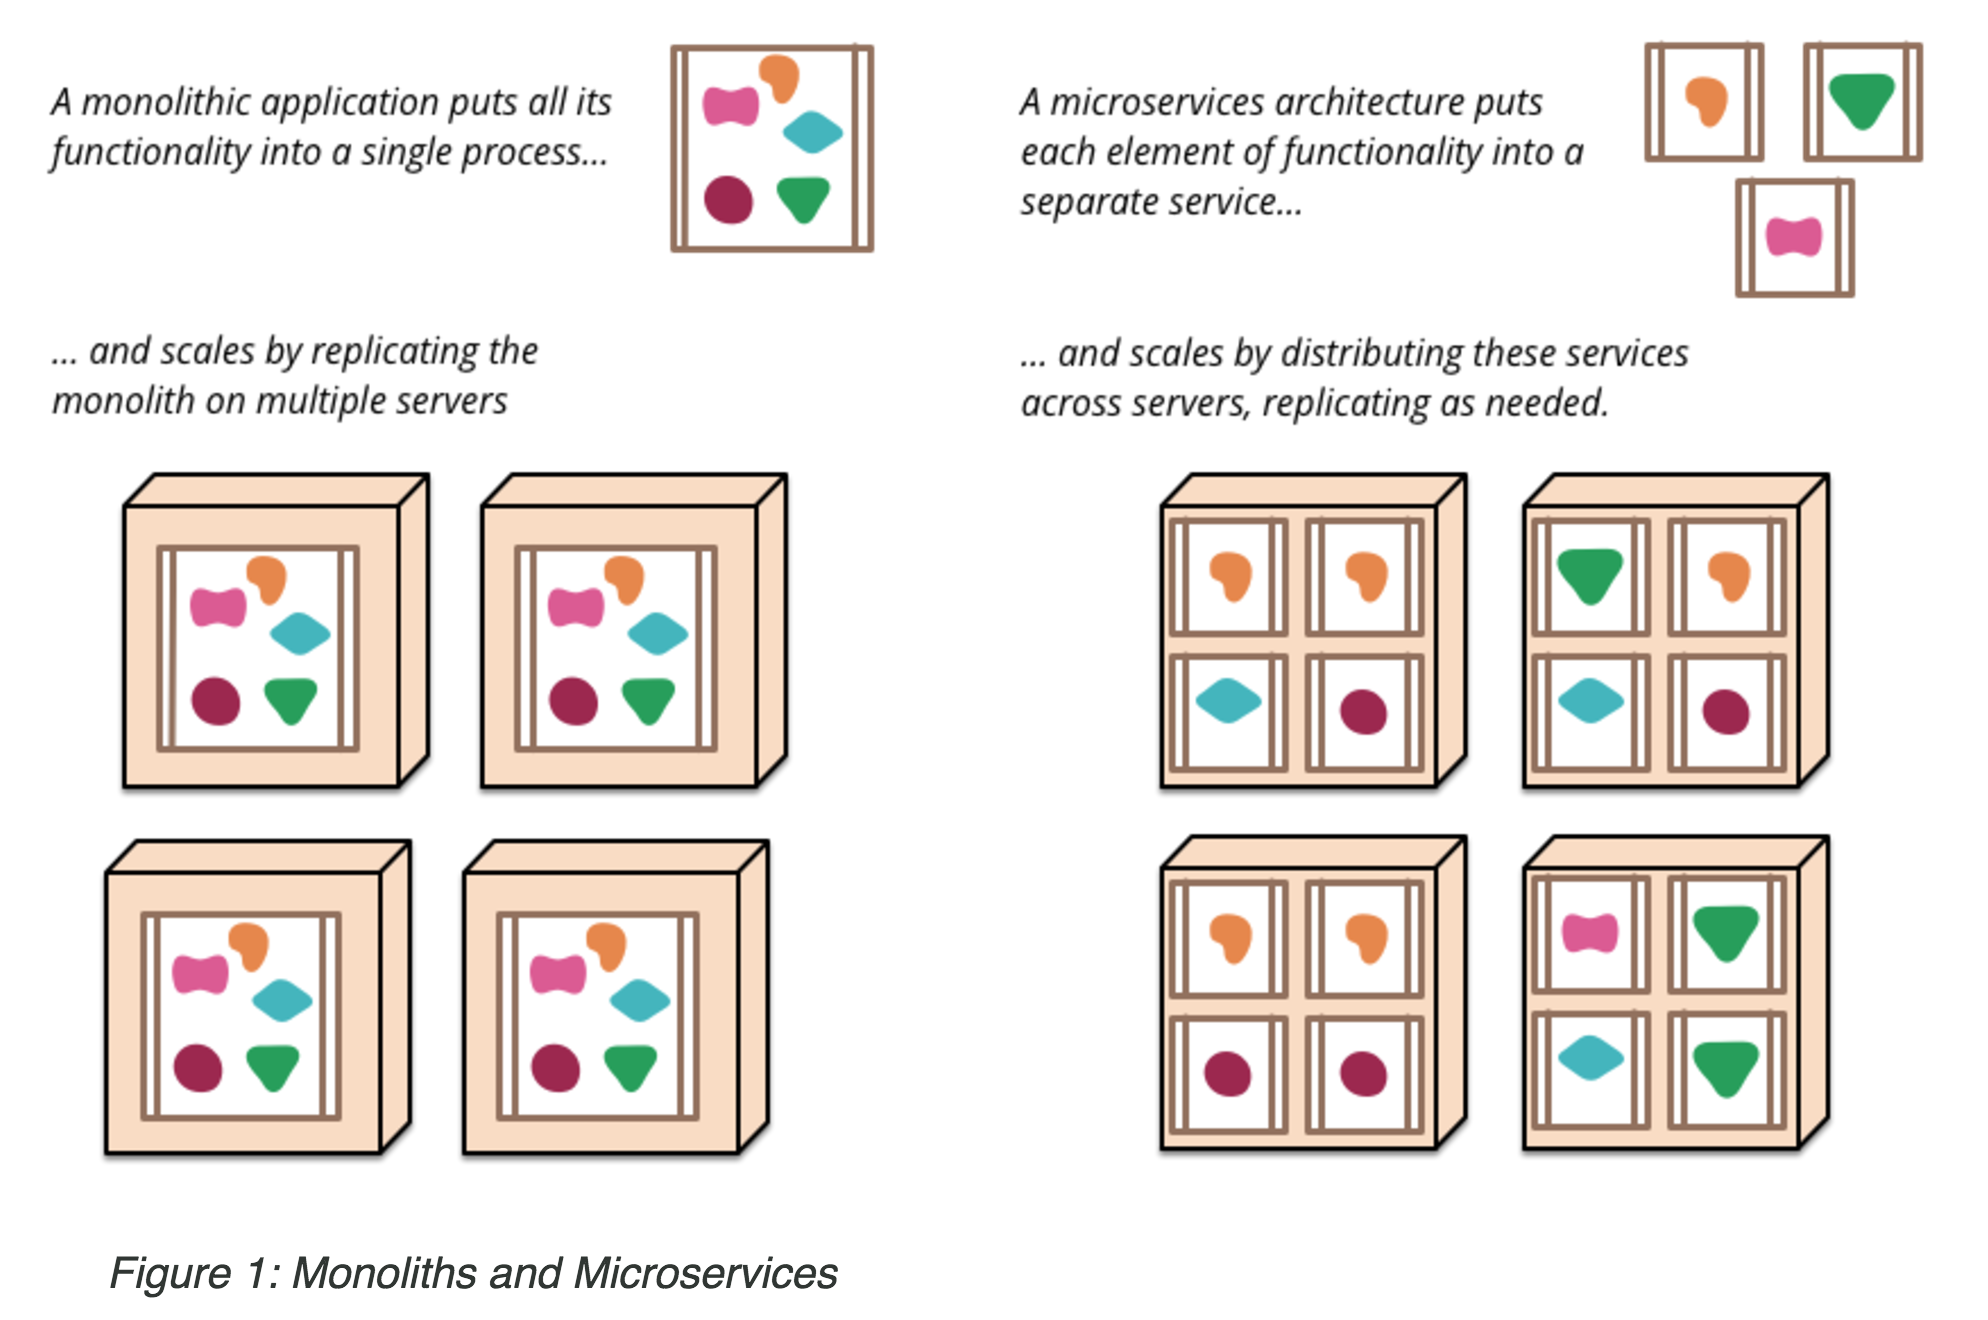
\includegraphics[scale=0.24]{architecture_microservice_definition}  
  \caption{Monolith and Microservice architectures compared}
  \label{fig:architecture_microservice_definition}
\end{figure}

"If you can do things that improve small projects, then that cumulative effect can be very significant on an enterprise, particularly since small projects often have disproportionate value. Indeed, one of the best things you can do is turn a large project into a small one by simplifying its architecture and process."

patterns of Enterprise Application Architectures page 4.


\subsection{Defining characteristics}
\note{
As the microservice architecture was created out of a need for reducing complexity and improving agility and reliability\cite[p.~68]{long2017cloud}, different companies started developing microservice architectures independently.
}
There is a series of defining characteristics for services in a microservice architecture, which should be followed to avoid pitfalls when utilizing microservices. These characteristics describe what teams utilizing microservices often times do, there is no definitive definition of what a microservice architecture is.

\subsubsection*{Componentization via Services}
Componentization is used to decouple parts of an application, so that a service is only responsible for limited amount of highly related functionality\cite{morgantini2013whatAreMicroServices}. The componentization can initially be created by analysing the domain and identifying bounded contexts\cite[p.~31]{newman2015microservices}, each bounded context contains information only important internally in the context. 
The external important information is therefore made available through a interface, while internally important information is hidden from outsiders, simplifying boundaries.

By using services for componentization, a explicit interface is created, hindering tight coupling between components. Explicit remote call mechanisms are often used to facilitate communication between components. Communication through remote calls incur some overhead, forcing communication interfaces to be on high abstraction levels, making them more awkward to use than in process calls.

\subsubsection*{Splitting around Business Capabilities}
Services are organized around business capabilities, by analysing the domain carefully, each service can be limited in size and functional requirements. Each service implements all functionality to fulfil the identified requirements for that part of the business area, potentially consisting of multiple processes, developed and deployed together. A service could implement a application process having a underlying database exclusively used for that application process\cite{fowler2014microservices}.

\subsubsection*{Well Defined and Simple Communication Channels}
Keeping logic out of the communication method is important when developing microservices. Inspired by UNIX implementation, microservice architecture tries to delegate the entire concern of applying logic to the service implementations. When a service receives a request it applies its logic as appropriate and produces a response. The communication is often done with HTTP request-responses, defining the communication interfaces with a REST protocol\cite{fowler2014microservices}.

\subsubsection*{Decentralized Governance}
By decentralizing governance and organising around business capabilities, each service can be build with technology that fits well with solving the problem.
\note{Kunne potentielt tilføje hvordan team skills også kan splittes ud, samt hvordan det gør teams i stand til at sidde forskellige steder og arbejde med det samme}

\subsubsection*{Decentralized Data Management}
Services often have their own data store, decentralizing data management. Each service has the data that is relevant for that service, and not more. 

\note{Potentielt gør brug af Martin Fowler artikel "PolyglotPersistence", der snakker om brug af NoSQL teknologier}

\subsubsection*{Automation of Deployment}
Microservices infer a lot of operational complexity, as there are many services to deploy and monitor. The use of infrastructure automation techniques is necessary, improving insight into the quality of newly developed software, and reduce the time it takes to move new features from development to production\cite{newman2015microservices}. This is often achieved with build pipelines know from Continous delivery (CD), a build pipeline is seen on figure \ref{fig:architecture_microservice_build_pipeline}.

\begin{figure}[!htb]
  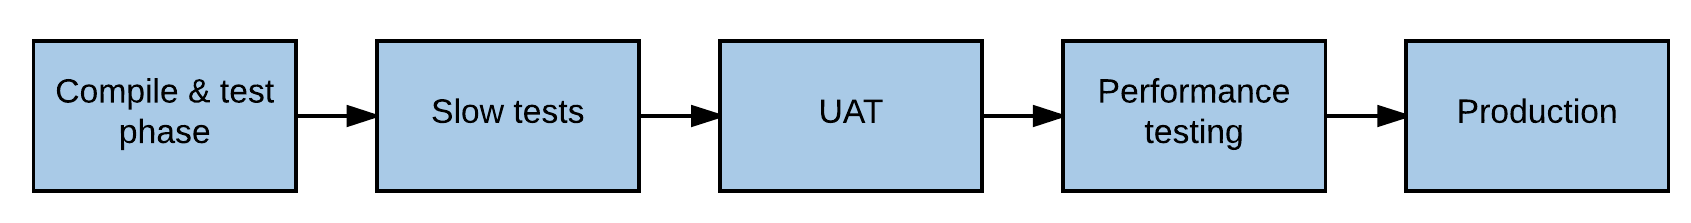
\includegraphics[scale=0.26]{architecture_microservice_build_pipeline}  
  \caption{Build pipeline(lend from Sam Newmann)}
  \label{fig:architecture_microservice_build_pipeline}
\end{figure}

\note {
\subsubsection*{Independently Deployable Services}
Each service is independently deployable, making it possible to add and update functionality in each service as needed.
}

\subsection{Derived qualities}
Microservices in it self presents a lot of benchmark benefits, giving possibility to control capacity, introduce redundancy and solve single point of failure issues, a microservice architecture improves overall application resilience if utilized correctly. At the same time microservices introduces additional complexity, because services has to communicate with dependent services using non-deterministic communication channels. This in turn has the effect of highlighting otherwise transparent challenges with integration points, causing engineers utilizing microservices to be more resilience aware, expecting failure between services. In a monolith implementation, a library dependency used in process might introduce new possible error states or undefined behaviour, but in this context software engineers tend to be less aware of the possible errors this dependency could incur. When having very clear interfaces with dependencies, engineers tend to take more precautionary measures. These measures are not directly measurable, but help create a more resilient system. 

\subsubsection*{Design for Failure}
A challenge with using services as components is the inherent complexity of communication over the wire, when two separate services need to communicate. In turn this highlights the existing pitfalls with every integration points, that exists even in a monolith architecture.

\subsubsection*{Sophisticated Real-Time Monitoring}
When designing many independent services, it is necessary to have sophisticated monitoring and logging, in order to control that services are running correctly. This enables engineers to know if any action needs to be taken to restore a fully functional system, or if service was automatically restored.


\section{Event-driven architecture}
\comment{This section is still in note form}
There are four patterns occurring in many of the systems where the word event-driven architecture.

Systems are often get very coupled because the different system depend on each other.

\section{Service discorvery}
C. Richardson, “Service discovery in a microservices architecture.” 
\url{https://www.nginx.com/blog/service-discovery-in-a-microservices-architecture/}


\section{Event notification}
It is a particular important part of the architecture. Subsystems communicate through events.

Applications subscribe to the events they are interested in, and react when an event comes along. 
By doing this you reverse dependencies.
Besides reversing dependencies, we now have a record that can be referred to and passed around, when an event happens. 'Bottling it op'.

What is the difference between events and commands. Events does not expect any specific reaction, but are just informing about change. Commands imply certain reaction to a event.

It allows us to hook up many different system up to events, without incurring change in existing applications. It easily allows to implement new features, without changing other

At the same time it removes easy observable flow. There is no code to look at, you have to debug.

\subsection{Event-carried State Transfer}
Downstream services duplicate the data they receive from events, removing the need for calls to the emitter. Less traffic is required, because more information is put into the events. Subscribing services can therefore deduct what to do from events, without contacting the emitter for additional data. The event therefore contains all the data that downstream systems want to have.

Downstream services therefore need to store the events they are interested in. 

It reduces the calls to the emitter, reducing traffic. Can improve availability, consumers are not directly tied to the emitter, the consumer has it's own data and can therefore continue operation if the emitter goes down.

This introduces lack of consistency. This is a less common pattern, but it can be a good one to utilize in some cases.

\subsection{Event Sourcing}
Changes are registered, by putting event on top of a event stack or log, the event is thereafter processed, updating the application state.

The Log can rebuild application state at any time.

In case of changes:
1. Event object is created - 'Address change' - pop into a seperate storage area
2. Process event - 'Change address'

Event sourcing works on customer state the way subversion works on code.

It is often a combination of all events and some 'snapshots'. Snapshots are sometimes done, 'closing out the year' ignoring events that has happened earlier, simplify the events, making it easier to reason about future events. Storage is therefore a mixture of events and snapshots. But you always want to be able to reason about the current state.

This pattern have several benefits:
Audit
Debugging, realy usefull to be able to go back and forth in state.
Historic state, if a error has occurred in the past, the difference it would make in current state can be calculated by going back and changing an event and calculating the difference.
Alternative state, you have a alternative to storing application state, by storing it in live memory. You still have to have an alternative store, so you can recreate state.

Disadvantages:
Unfamiliar, harder to work with
External system, gets a bit more complex, cannot ask the system for events again. Therefore a replay mechanism has to be made, to be able to restore application state. Has to save events.
Event Schema, how are events stored, so they can be replayed while the application that processes them is changed around them.
Identifiers, Traps when trying to make it possible to replay application state.
Potential disadvantages:
Asynchrony, adds complexity as it is introduced to handle emitting and handling events. It does not have to be used though.
Version, It can be hard to reason about. If application state structure is changed, can the application the still process year old events. Snapshots can be cut down two one day, so this is not a problem.

Pros and cons. Advantages and disadvantages.

\subsection{Command Query Responsibility Segregation}
Seperate pieces of software components that read and write to the central store.

Command model, write the model. It is only used when making updates.

Query model, 

It is appropriate pattern, but seems to 


